\providecommand{\relativeRoot}{../..}
\documentclass[\relativeRoot/main.tex]{subfiles}
\graphicspath{
    {\subfix{./figures/}}
}


\begin{document}

\section{Head and Neck Squamous Cell Carcinoma}
\label{sec:intro:hnscc}

\begin{figure}
    \centering
    \begin{tikzpicture}[very thick, line cap=round]
        \node[above left, inner sep=0pt] (image) at (0,0) {
            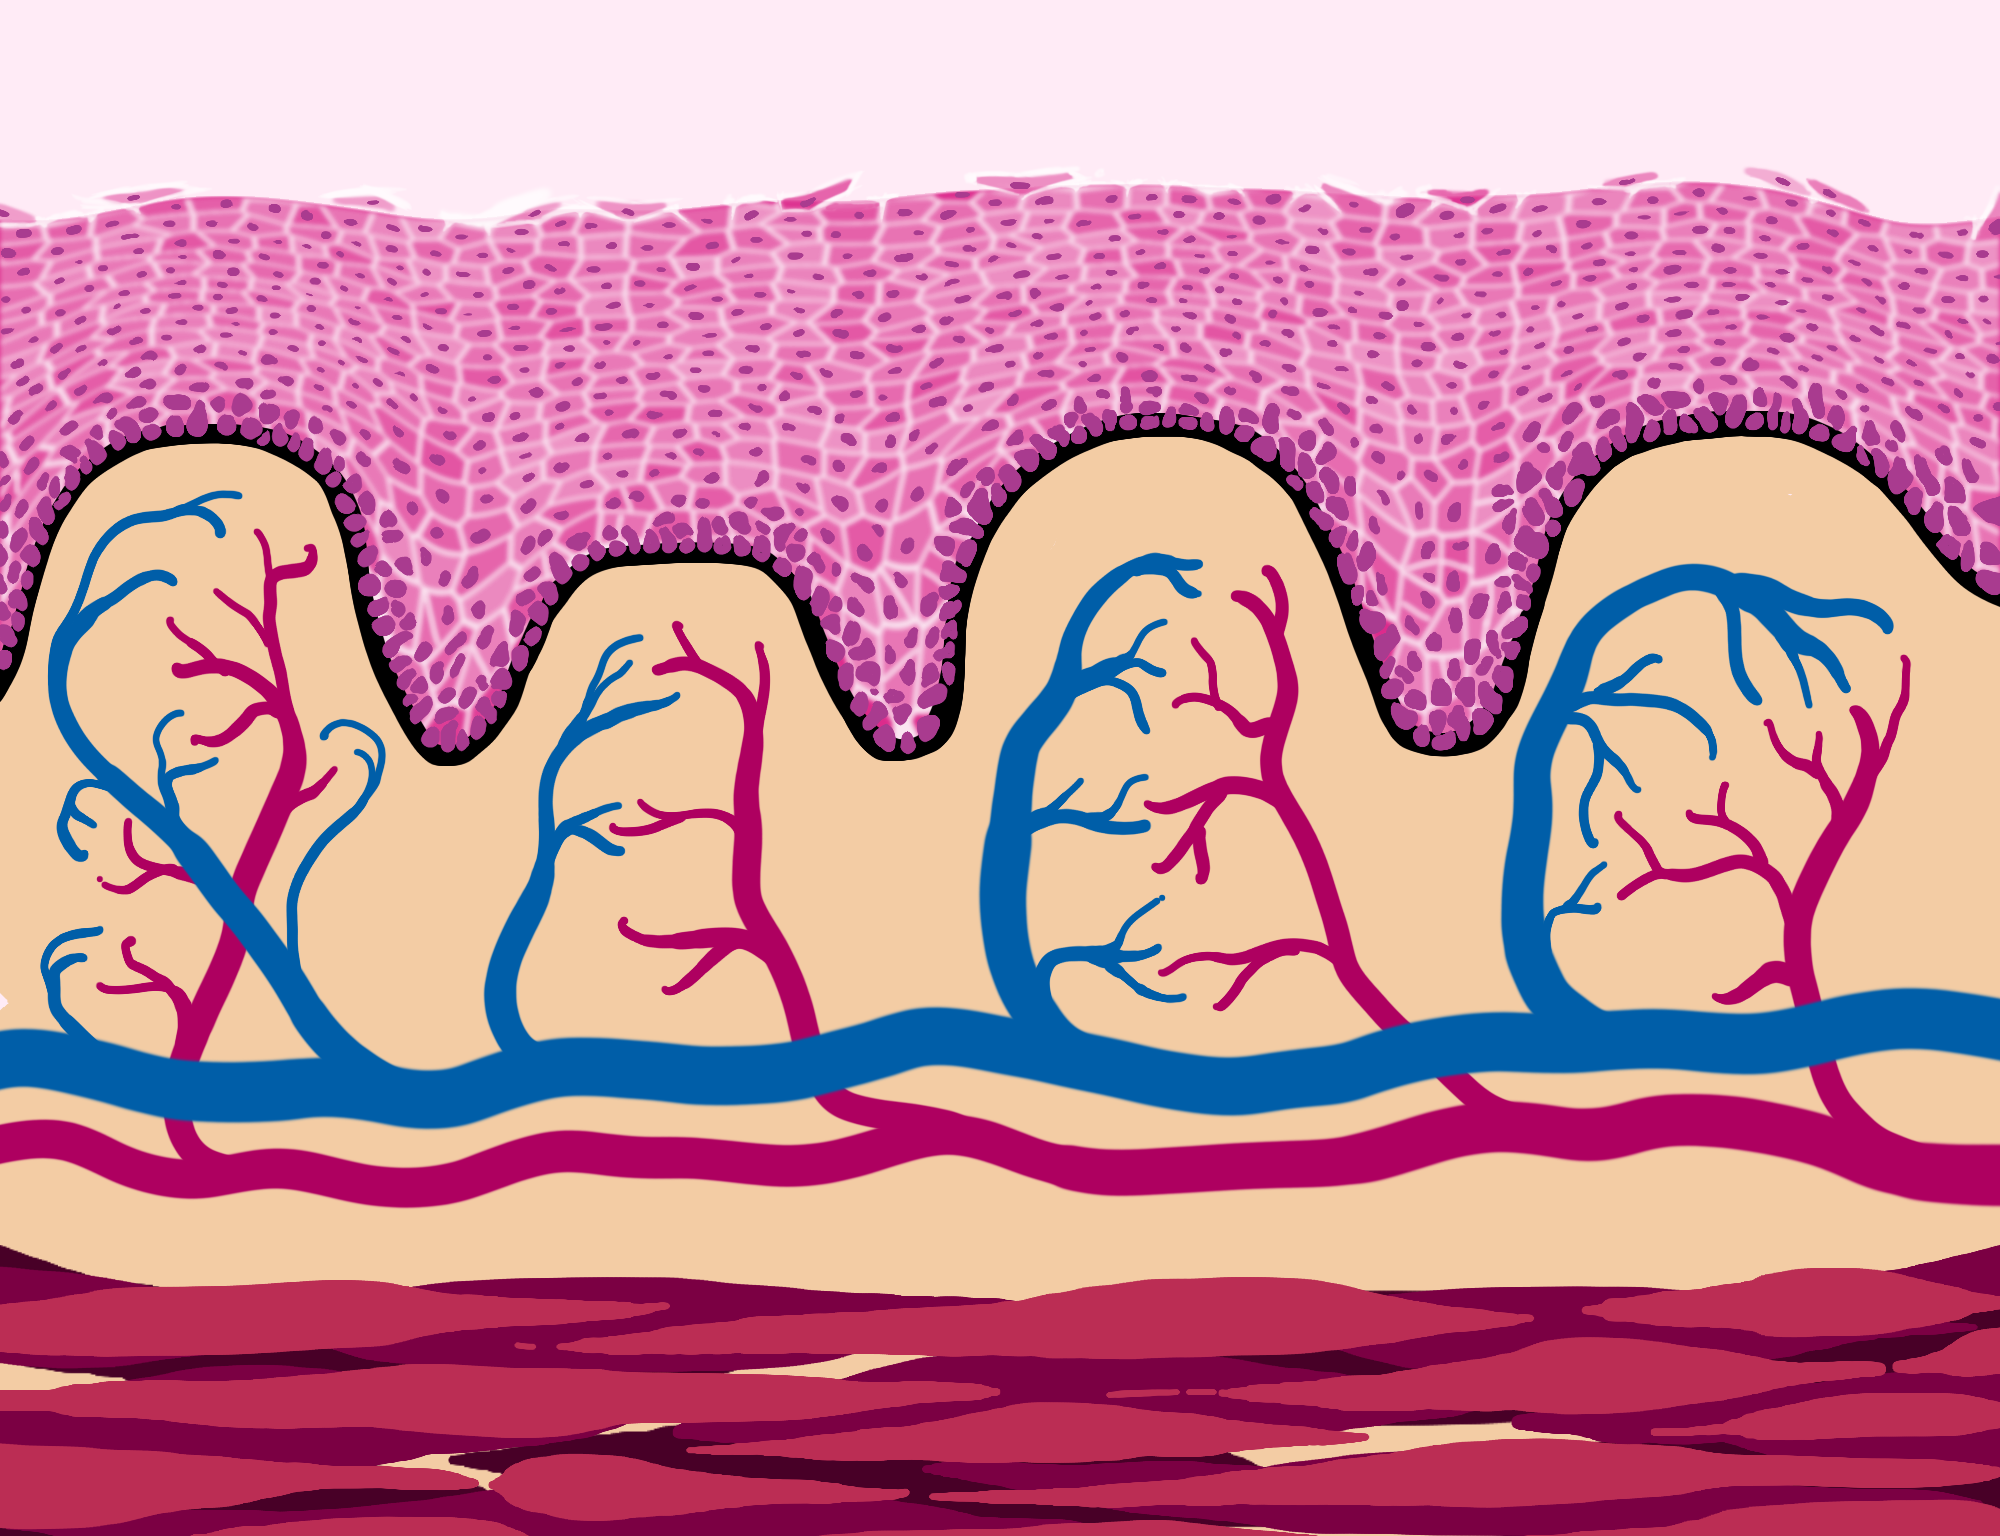
\includegraphics[width=0.8\textwidth]{figures/mucosa.png}
        };

        \draw[
            decorate,
            decoration={
                brace,
                raise=5pt,
                amplitude=5pt,
                mirror,
            },
        ] (0,0) -- (0,1.7)
        node[
            pos=0.5,
            right=10pt,
            text width=0.18\textwidth,
            align=left,
            execute at begin node=\setlength{\baselineskip}{10pt}
        ]{muscle layer};
        \draw[
            decorate,
            decoration={
                brace,
                raise=5pt,
                amplitude=5pt,
                mirror,
            },
        ] (0,1.8) -- (0,5.4)
        node[
            pos=0.5,
            right=10pt,
            text width=0.18\textwidth,
            align=left,
            execute at begin node=\setlength{\baselineskip}{10pt}
        ]{submucosa and lamina propria};
        \draw (5pt,5.5) -- (10pt,5.5)
        node[
            right,
            text width=0.18\textwidth,
            align=left,
            execute at begin node=\setlength{\baselineskip}{10pt}
        ]{basement layer};
        \draw[
            decorate,
            decoration={
                brace,
                raise=5pt,
                amplitude=5pt,
                mirror
            }
        ] (0,5.6) -- (0,7.8)
        node[
            pos=0.5,
            right=10pt,
            text width=0.18\textwidth,
            align=left,
            execute at begin node=\setlength{\baselineskip}{10pt}
        ]{stratified squamous cells};
    \end{tikzpicture}
    \caption[
        Schematic of the buccal mucosa layers
    ]{
        Schematic showing the layers of the oral mucosa (e.g. on the inside of the cheeks). From bottom to top the displayed layers are
        \begin{enumerate*}[label={(\arabic*)}]
            \item muscle tissue,
            \item submucosa and lamina propria with circulatory vessels,
            \item a black basement layer and
            \item the epithelium consisting of stratified, squamous cells
        \end{enumerate*}.
    }
    \label{fig:intro:mucosa}
\end{figure}

All body surfaces and cavities are covered in a type of tissue called \emph{epithelium}. For example, both the skin and the lungs are lined with epithelial cells. Of those cells, three different basic types can be distinguished:
\begin{enumerate*}[label={(\arabic*)}]
    \item \textbf{Squamous} (from \emph{squama}, Latin for ``scale'') cells are flat and thin, while 
    \item \textbf{cuboidal} cells are approximately as thick as they are wide and lastly
    \item \textbf{columnar} epithelial cells are column-like and hence much taller than wide
\end{enumerate*}.
They often have a hexagonal shape when viewed from above (meaning perpendicular to the surface they cover) and are close-packed with little to no intercellular space \cite{marieb_human_1995}.

Malignancies -- or more precisely \emph{malign neoplasms} -- that develop in squamous cells of the epithelium are called \gls{scc}. They are caused by specific mutations in the epithelial stem cells, which are responsible for creating new functional squamous cells. In \cref{fig:intro:mucosa} we show a basic schematic of how parts of the oral mucosa are layered. There, the origin of \gls{scc} would usually be located on the black line we have labelled \emph{basement layer}, to which the stem cells of the epithelium are attached.

As many parts of the human body are covered by some type of epithelium, there exists a respective variety of locations where \glspl{scc} can arise. E.g., it is common in the lung, skin or the vagina. But it may also arise in the mucosa (see \cref{fig:intro:mucosa}) inside the mouth and upper respiratory tract. In that case, the malignancy is termed \gls{hnscc}.

\gls{hnscc} is the most common type of head and neck cancer, and among the ten most common types of cancer worldwide with an incidence of almost 900,000 new cases in 2018, of which 450,000 resulted in deaths. \cite{johnson_head_2020,ferlay_estimating_2019,bray_global_2018}. Air pollutants, tobacco and alcohol abuse have been linked to an increased risk for \gls{hnscc} \cite{johnson_head_2020,wong_cancers_2014}, as well as an infection with the \gls{hpv}, especially the subtype \gls{hpv}-16 \cite{hennessey_human_2009}.

\end{document}
